\documentclass[12pt,a4paper]{article}

\usepackage[utf8]{inputenc}
\usepackage[russian]{babel}
\usepackage[OT1]{fontenc}
\usepackage{amsmath}
\usepackage{amsfonts}
\usepackage{amssymb}
\usepackage{graphicx}
\usepackage{tikz}
\usepackage{pgfplots}
\usepackage[export]{adjustbox}
\usepackage{wrapfig}
\usepackage[left=2cm,right=2cm,top=2cm,bottom=2cm]{geometry}
\usepackage{setspace}


\begin{document}

\title{
2.2.1.

Исследование взаимной диффузии газов.
\author{Семёнов Андрей Б02-016}
}
\date{8 апреля 2021г.}

\maketitle

\newpage

\textbf{Цель работы:}
\begin{enumerate}
    \item Регистрация зависимости концентрации гелия в воздухе от времени с помощью датчиков теплопроводности при разных начальных давлениях смеси газов
    \item Определение коэффициента диффузии по результатам измерений
\end{enumerate}

\textbf{В работе используются:}
\begin{itemize}
    \item измерительная установка
    \item форвакуумный насос
    \item баллон с газом (гелий)
    \item манометр
    \item источник питания
    \item магазин сопротивлений
    \item гальванометр
    \item программа по дополнительнуому описанию эксперимента
\end{itemize}


\section{Теоретические сведения}
\begin{enumerate}
\item {\sl Диффузия} $-$ самопроизвольное перемешивание молекул, происходящее вследствие их хаотичного теплового движения. При перемешивании молекул разного сорта говорят о {\sl взаимной} (или {\sl концентрационной}) диффузии.

В системе, состоящей из двух компонентов, плотность потока вещества в результате взаимной диффузии описывается законом Фика:
\begin{center}
$j_a = -D_ab\frac{\partial n_a}{\partial x}$, $j_b = -D_ba\frac{\partial n_b}{\partial x}$,
\end{center}
где $D_{ab} = D_{ba} = D$ - {\sl коэффициент взаимной диффузии} компонентов, $j_{a},j_{b}$ = плотности потока частиц соответствующего сорта (количество частиц, пересекающих единичную площадку в единицу времени).\\
В работе исследуется диффузия примеси лёгкого газа (гелия) на фоне воздуха, поэтому концентрация воздуха в опыте значительно больше концентрации гелия, и её относительное изменение незначительно. В процессе работы будет описываться только диффузия примеси гелия на стационарном фоне воздуха.\\

\item Проведём теоретическую оценку величины коэффициента взаимной диффузии. В работа мала концентрация гелия, более того, масса атомов гелия много меньше массы молекул, составляющих воздух. При таких условиях перемешивание газов в эксперимента можно рассматривать как диффузию гелия на стационарном форне воздуха. Тогда коэффициент диффузии приблизительно равен
\begin{center}
$D = \frac{1}{3}\lambda \bar v$,
\end{center}
где $\lambda$ - длина свободного пробега частиц гелия, $\bar v = \sqrt{\frac{8kT}{\pi m}}$ - их средняя тепловая скорость. В общем случае необходимо считать $\lambda = \frac{1}{n_{\Sigma \sigma}}$, где $n_{\Sigma} = n_{He} + n_{B} = \frac{P_{\Sigma}}{kT}$ - полная концентрация частиц, $\sigma$ -  среднее сечение столкновения частиц гелия с воздухом. Также  $\bar v = \sqrt{\frac{8kT}{\pi \mu}}$ - средняя относитель. Таким образом, теоретическая оценка предполагает, что коэффициент диффузии не зависит от пропорция элементов, а обратно пропорционален давлению $D \propto \frac{1}{P_{\Sigma}}$.
\item  Рассмотрим процесс выравнивания концентрации в установке, она зависит от координат и времени во всей установке. Объём соединительной трубки мал по сравнению с с объёмами сосудов. Поэтому концентрации газов можно считать постоянной по всему объёму сосудов; считаем, что процесс выравнивания происходит только за счёт диффузии в трубке и является стационарным (так как считаем стационарным поток частиц). Величина этого стационарного потока $J = -DS\frac{\partial n}{\partial x}$, и он одинаковый во всём сечении трубки, тогда $n(x)$ - линейная функция координаты и $\frac{dn}{dx} = \frac{\Delta n}{l}$ (l - длина трубки), получаем 
\begin{center}
$J = -DS \frac{n_{1}-n_{2}}{l}$.
\end{center}
Предположим, что установился линейный профиль концентрации и полученное соотношение справедливо в любой момент времени. Получаем {\sl квазистационарное} приближение зависимости концентраций $n_1$ и $n_2$ от времени.
\item Через $\Delta n_1$ и $\Delta n_2$ обозначим изменения концентрации в объёмах $V_1$ и $V_1$ за время $\Delta t$. Тогда $V_1 \Delta n_1$ - изменение количества компонента в объёме $V_1$, а $V_2 \Delta n_2$ - изменение количества этого компонента в объёме $V_2$. По закону сохранения вещества следует, что $V_1 \Delta n_1 + V_2 \Delta n_2 = const$, поэтому $V_1 \Delta n_1 = - V_2 \Delta n_2$. Эти изменения происходят вследствие диффузии, поэтому 
\begin{center}
$V_1 \Delta n_1 = - V_2 \Delta n_2 = J \Delta t = -DS \frac{n_1-n_2}{l} \Delta t$
\end{center}
Делим равенство на $\Delta t$
\begin{center}
$V_1 \frac{dn_1}{dt} = -DS\frac{n_1-n_2}{l}$, $V_2 \frac{dn_2}{dt} = -DS\frac{n_1-n_2}{l}$
\end{center}
Делим первое уравнение на $V_1$, второе на $V_2$, вычтем равенства друг из друга:
\begin{center}
$\frac{dn_1}{dt}- \frac{dn_2}{dt} = - \frac{n_1-n_2}{l}DS(\frac{1}{V_1} +\frac{1}{V_2} )$.
\end{center}
Введём новую переменную $\Delta n = n_1-n_2$, проинтегрируем уравнение, получим
\begin{center}
$\Delta n = \Delta n_{0}\cdot e^{-t/\tau}$,
\end{center}
где $\Delta n_0$ - разность концентраций примеси в начльный момент времени, а
\begin{center}
$\tau = \frac{V_1 V_2}{V_1 + V_2} \frac {l}{SD}$.
\end{center}
Видим, что разность концентраций убывает по экспоненциальному закону и тем быстрее, чем меньше $\tau$ - величина, определяющаяся геометрическими параметрами установки и величиной коэффициента диффузии.
\item Для проверки применимости квазистационарного течения убедимся, что время $\tau$ много больше характерного времени диффузии одной частицы вдоль трубки длиной $l$: $t_{diff} \sim \frac{l^2}{D} \ll \tau$.

\item Для измерения концентраций применяются датчики теплопроводности $D_1$ и $D_2$ (см. рис. 1) и используется зависимость теплопроводности газовой смеси от её состава. Тонкая проволока радиуса $r$, протянутая вдоль оси цилиндра радиуса $R$, нагревается током. Тепло от проволоки к стенке цилиндра передаётся главным образом вспледствие теплороводности газа, находящегося внутри цилиндра. Количество тепла переданного стенке цилиндра в единицу времени, определяется по формуле 
\begin{center}
$Q = \varkappa \frac{2\pi L}{ln (R/r)}(T_1-T_2)$,
\end{center}
где $\varkappa$ - теплопроводность, $L$ - длина нити, $T_1, T_2$ - температуры проволочки и стенки. При $Q = const$ температура проволоки и её сопротивление определяются теплопроводностью газа и, следовательно, его составом. Для измерения разности концентраций газов используется  
мостовая схема, представленная на рис. 2 (см. пункт 4).

\item В процессе диффузии разность концентраций убывает по экспоненциальному закону. По тому же закону изменяются во времени показания гальванометра:
\begin{center}
$U = U_{0}\cdot e^{-t/\tau}$
\end{center}
Измеряя экспериментально зависимость $U(t)$, можно получить характерное время процесса $\tau$, откуда определить коэффициент диффузии D.
\end{enumerate}

\section{Экспериментальная установка}

\begin{enumerate}
\item Общий вид конструкции установки приведён на рис. 1. Установка состоит из двух сосудов $V_1$ и $V_2$, соединённых краном $K_3$, форвакуумного насоса Ф.Н. с выключателем Т, манометра М и системы напуска гелия, состоящей из кранов $K_6, K'_6, K_7$. Кран $K_5$ позволяет соединять форвакуумны насос либо с установкой, либо с атмосферой. Сосуды $V_1$ и $V_2$ соединены трубкой длины $l$ и сечения $S$. Сосуды заполнены смесь двух газов при одинаковом давлении, но с различной концентрацией компонентов. Вследствие взаимной диффузии концентрации каждого из компонентов с течением времени выравниваются Между форвакуумным насосом и краном $K_5$ вставлен предохранительный баллон, защищающий кран и установку при неправильной её эксплуатации от попадания форвакуумного масла из насоса. Сосуды $V_1$ и $V_2$ можно соединять как с системой напуска гелия, так и с форвакуумным насосом. Для этот служат краны $K_1, K_2, K_4, K_5$. Манометр М регистрирует давление газа, до которого заполняют тот или иной сосуды. Кран $K_4$ изолирует форвакуумный насос от установки. Для подачи воздуха в установку служит кран $K_5$. Дополнительный кран $K'_6$ служит для вакуумной изоляции установки от системы подачи гелия. Краны $K_4, K_5, K'_6$ обладают повышенной вакуумплотностью и хорошо изолируют установку от протечек.

\begin{figure}[h]
    \centering
    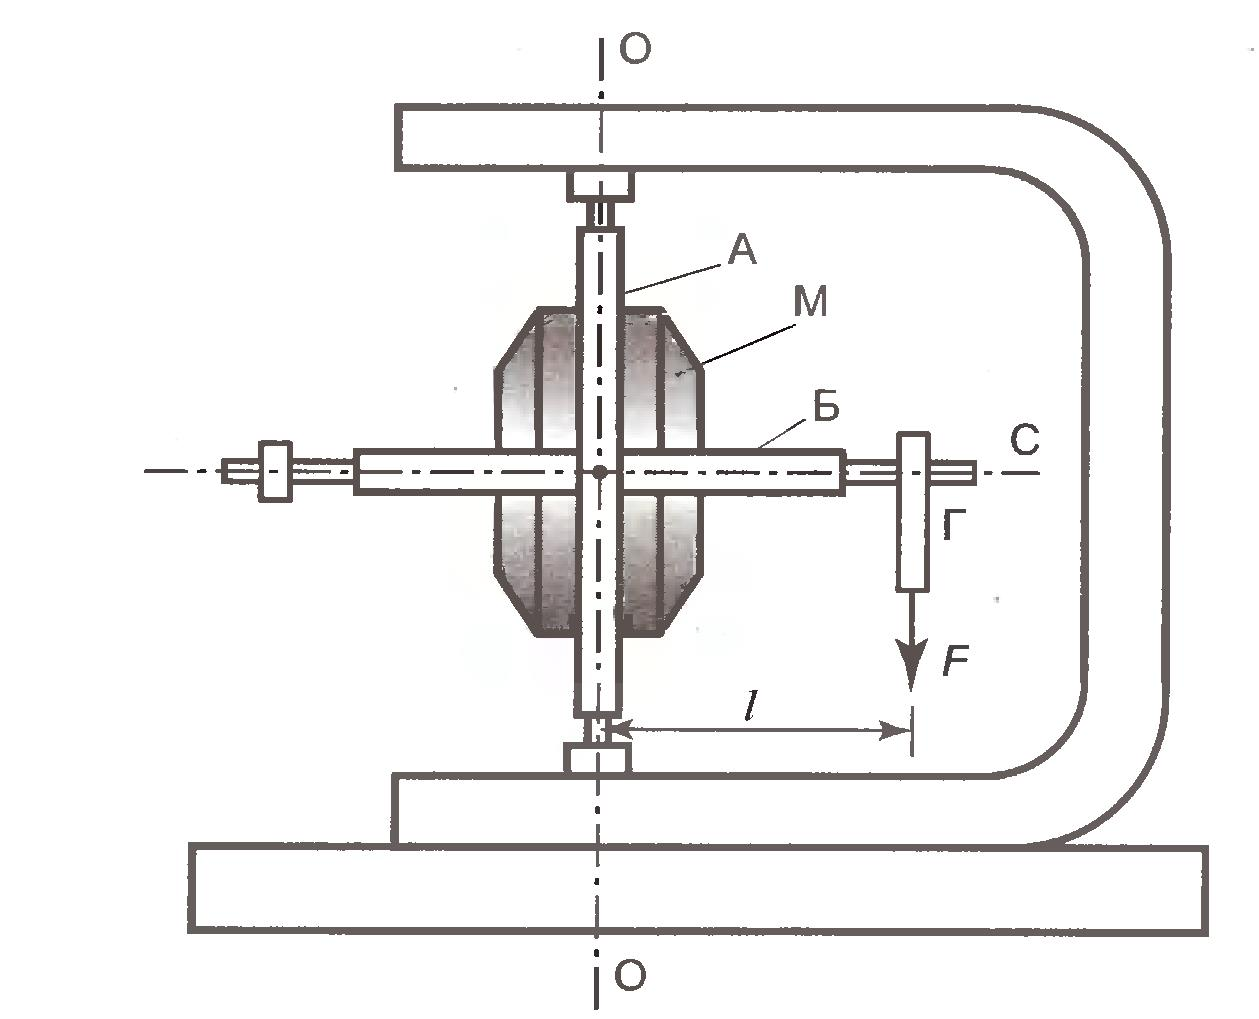
\includegraphics[width=7.5 cm]{facility.PNG}
    \caption{Установка для исследования взаимной диффузии газов}
    \label{fig:vac}
\end{figure}

\item Для измерения разности концентраций газов используется мостовая схема, представленная на рисунке 2. \\
Здесь $D_1, D_2$ - датчики теплопроводности, расположенные в сосудах $V_1$ и $V_2$. Сопротивления $R_1, R_2, R$ служат для установки прибора на нуль (балансировка моста). В одну из диагоналей моста включен гальванометр, к другой подключается небольшое постоянное напряжение. Сопротивления $R_1$ и $R_2$ спарены (их подвижные контакты находятся на общей оси) и изменяются одновременно при повороте ручки грубой регулировки. Точная балансировка выполняется потенциометром R. Балансировку необходимо проводить перед каждым экспериментом заново: при этом установка заполняется чистым газом (воздухом без гелия) при давлении, близком «рабочему» (при котором затем будут проводится измерения).

 Мост балансируется при заполнении сосудов (и датчиков) одной и той же смесью. При заполнении сосудов смесями различного состава возникает «разбаланc» моста. При незначительном различии в составах смесей показания гальванометра, подсоединённого к диагонали моста, будут пропорциональны разности концентраций примеси: $U \propto \Delta \varkappa \propto \Delta n$
 
\begin{figure}[h]
    \centering
    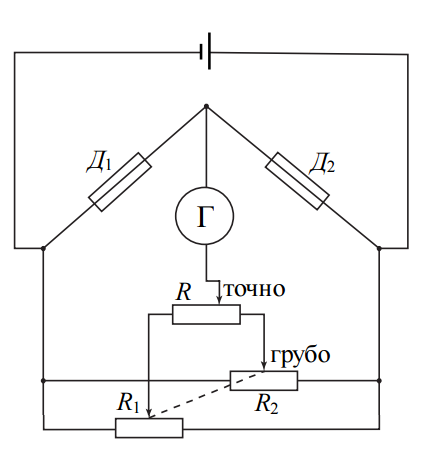
\includegraphics[width=5.5 cm]{scheme.PNG}
    \caption{Мостовая схема с датчиками теплопроводности для измерения разности концентраций газов}
    \label{fig:vac}
\end{figure} 

\item Гелий содержится в баллоне (не изображен на рис. 1) под давлением, превышающим атмосферное. Для предотвращения избыточного расхода гелия и
его неконтролируемого проникания в установку предусмотрен металлический кран (К7), отделяющий её от баллона с гелием. Его открывают только на
время непосредственного заполнения установки гелием, остальное время он должен быть закрыт. Для подачи малых порций гелия предусмотрен двухходовый кран с дозатором (рис. 4). При повороте рычажка Р в положение I гелий в небольшом количестве поступает в дозатор (если открыт К7), а при повороте Р в положение II порция из дозатора поступает в установку.

\begin{figure}[h]
    \centering
    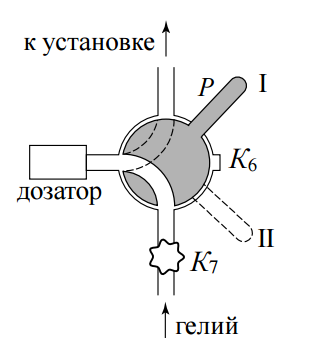
\includegraphics[width=5.5 cm]{crane.PNG}
    \caption{Кран $K_6$}
    \label{fig:vac}
\end{figure} 

\end{enumerate}

\section {Выполнение работы}

\end{document}
